% !TEX root = catron-dissertation.tex
\chapter{Introduction}
The best possible performance of a directed energy system whether airborne or ground based in the far-field is the diffraction-limited case.
The far-field intensity of a diffraction-limited beam in represented by $I_0$ and defined in Equation \ref{eqn:01_farfield_intensity},
\begin{equation}
  I_0 = \left(\frac{kAp^2}{8z}\right)^2
  \label{eqn:01_farfield_intensity}
\end{equation}
where $k$ is the wavenumber of the beam, $Ap$ is the aperture size, and $z$ is the distance from the aperture to the far-field.
Figure \ref{fig:01_farfield_intensity} show the far-field diffraction-limited intensity of a beam as the wavelength of the beam is varied and normalized by $I_0$ at 1$\mu$m.
\begin{figure}
  \centering
  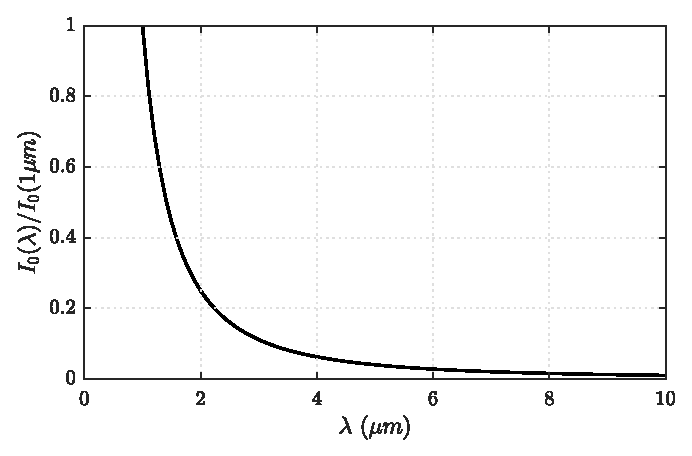
\includegraphics{../matlab/01_introduction/farfield_intensity.eps}
  \caption{Diffraction-limited far-field intensity of a beam normalized by the performance at 1$\mu$m.}
  \label{fig:01_farfield_intensity}
\end{figure}
As the wavelength of an outgoing beam decreases the diffraction-limited performance greatly improves proportional to $\lambda^{-2}$.
This provides a strong desire to move towards shorter wavelengths to take advantage of significantly increased diffraction-limited performance.

While diffraction-limited provides the best possible performance, real systems will however have reduced performance.
The ratio of actual on target intensity, $I(t)$, to diffraction-limited intensity is the Strehl ratio, $\textrm{SR}$, shown here using the large aperture approximation,
\begin{equation}
  \textrm{SR}(t) = \frac{I(t)}{I_0} \approx \exp\left\{-\left[\frac{2\pi \textrm{OPD}_{rms}(t)}{\lambda}\right]^2\right\}
  \label{eqn:01_strehl_ratio}
\end{equation}
where $\textrm{OPD}_{rms}(t)$ is the spatial root-mean-square of the optical path difference across the aperture.
The Airborne Laser Laboratory (ALL) which ran from the 1970s to early 1980s used a 10.6 $\mu$m laser and had an estimated Strehl ratio of 95\%\cite{Jumper-2013-8KtN3pue}.
Figure \ref{fig:01_strehl_ratio} shows a hypothetical case of varying the source wavelength while maintaining the same optical disturbance of ALL.
\begin{figure}
  \centering
  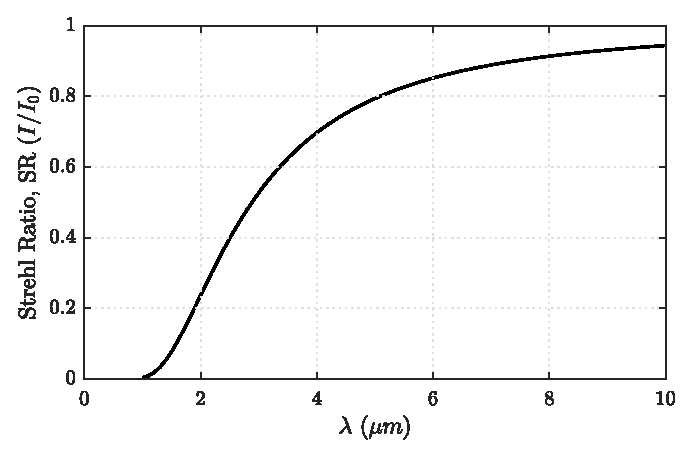
\includegraphics{../matlab/01_introduction/strehl_ratio.eps}
  \caption{Strehl ratio due to the $\textrm{OPD}_{rms}$ of the Airborne Laser Laboratory at various laser wavelengths.  ALL had an estimated Strehl ratio of 95\% with its 10.6 $\mu$m laser.}
  \label{fig:01_strehl_ratio}
\end{figure}
By changing the laser source to 1 from 10 $\mu$m nets a 100 times increase in diffraction-limited performance, the actual on target intensity drops to practically zero if using a system with the same optical disturbances present on ALL.

As future airborne directed energy systems are developed, their optical disturbances ($\textrm{OPD}_{rms}$) will need to be greatly reduced in order to achieve desired on target performance criteria.
These systems when tested on the ground in wind tunnels will see optical disturbances that are inherent to the test facility that may be on the order of the optical disturbances of the system its self.
This research will look at the optical disturbance contamination that comes from the acoustic waves that travel inside of a wind tunnel.
